\chapter{Experiments}\label{ch:exp}

In this chapter,
we present experiments demonstrating the performances of all the components developed in the previous chapters.

\section{Scalability of sparse naive Bayes}\label{sec:snb_criteo}

This experiment is not related to the knockoffs framework,
but shows the very good scalability of sparse naive Bayes
presented in Section~\ref{sec:snb}.
As part of the Kaggle competition \emph{Display Advertising Challenge}\footnote{
    The Kaggle competition can be found at
    \href{https://www.kaggle.com/c/criteo-display-ad-challenge}{this address}.
}
in mid-2014, CriteoLabs shared log data collected over one week\footnote{
    The competition's dataset can be downloaded at
    \href{https://labs.criteo.com/2014/02/download-kaggle-display-advertising-challenge-dataset/}{this address}.
}
whose features were undisclosed for confidentiality purposes.
Main characteristics of this dataset can be found in Table~\ref{tab:criteo_dataset}.
\begin{table}[!htb]
    \centering
    \setlength{\tabcolsep}{2pt}
    {\small
        \begin{tabular}{|c|c|c|c|c|}\hline
        \textbf{Samples} & \textbf{Total features} & \textbf{Numerical features} & \textbf{Categorical features} & \textbf{Features after encoding}\\ \hline
        $45\,840\,617$ & $39$  & $13$ & $26$ & $33\,762\,590$ \\ \hline
        \end{tabular}
    }%
    \caption[short]{
        Criteo dataset characteristics.
        Even though the number of features is small,
        most categorical features have millions of categories.
        It makes the training of predicting models particularly challenging as it requires several
        dozens of GB of memory.
    }
    \label{tab:criteo_dataset}
\end{table}
It consists in roughly $45$ millions of display ads with 39 features,
and a boolean label describing whether or not the ad was clicked by a customer.
Among these 39 features, 26 are categorical and a classical one-hot encoding would end up in millions of features.
This makes the Criteo dataset challenging, as it doesn't fit in the random-access memory after encoding,
and potentially not in the mass storage of a standard computer either (if a simple one-hot encoding is done).
Even on a small subset of covariates, say 10\%,
selecting important features using the Lasso or $\ell_1$-penalized logistic regression isn't realistic.

Figure~\ref{fig:criteo_hash_elbow} shows the optimal value of~\ref{eq:msnb} on this dataset as a function
of the sparsity level $k$.
All the computations are done on a standard workstation (16GB, Intel Core i7 3.60GHz $\times$ 8).
Sparse naive Bayes requires data averages to run,
i.e.\ the sums of the negative and of the positive points.
This part is time consuming but once these sums are computed they can be reused for any sparsity level $k$.
Using the accelerated Python interpreter PyPy, we obtain these averages in around 20 minutes.
Then, SNB optimal values are computed for 1200 log-spaced points in 1 hour,
using a Python and NumPy implementation of SNB\footnote{
    An implementation of sparse naive Bayes can be found~\href{https://github.com/aspremon/NaiveFeatureSelection}{here}.
}.
In this situation, what makes SNB particularly appealing is the fact that at no moment we need to load the full dataset
in memory.
We are only computing data averages whose shape are much smaller than the full matrix.
Note also that most tasks could even be distributed to speed up the computations.
\begin{figure}
    \centering
    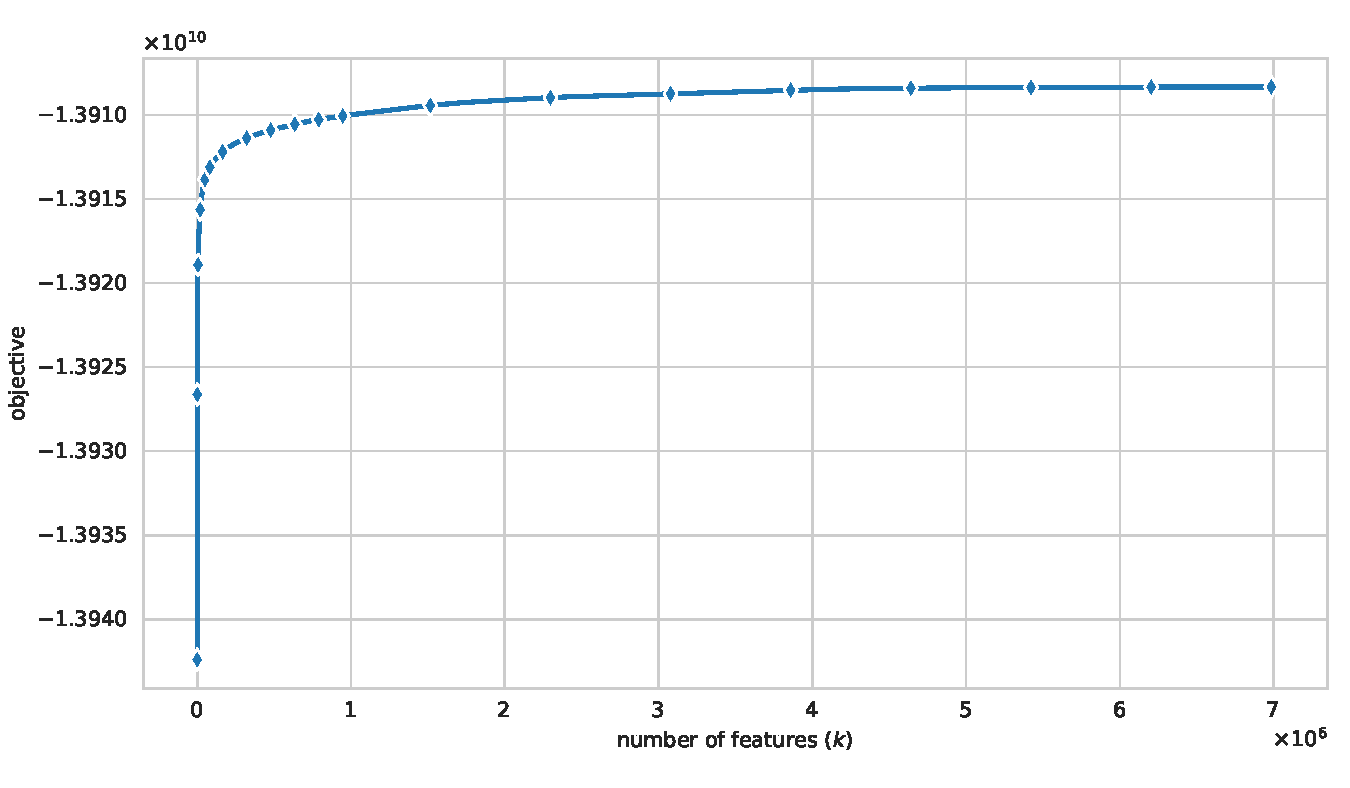
\includegraphics[width=0.75\linewidth, height=0.4\linewidth]{figures/criteo_hash_elbow.pdf}
    \caption{
        Optimal value of the~\ref{eq:msnb} optimization problem on the Criteo dataset
        as a function of the sparsity parameter $k$.
        Only 1--2 millions of the features explain most of the target vector (elbow heuristic).
    }
    \label{fig:criteo_hash_elbow}
\end{figure}
Refer to Appendix~\ref{sec:criteo_data} for more details regarding the experiment setup.

\section{Statistical power comparison}\label{sec:power_comparison}

\section{FDR control on genetic data}\label{sec:genetic_data}

We experiment the high-dimensional knockoff selection pipeline
described in the previous chapters to genetic data.
We preprocess the dataset ARCHS4\footnote{
    Data available at \href{https://amp.pharm.mssm.edu/archs4/download.html}{this address},
    under the filename \texttt{human\_matrix.h5 v8}.
}
which contains the gene expression levels of thousands of patients,
along with characteristics regarding their medical conditions.
We extract healthy patients,
and those who suffer from lung cancer.
We end up with roughly $2\,500$ patients and $35\,000$ features.
Due to the large number of features,
the tools developed in the previous chapters are particularly suited in this situation.
\begin{table}[!htb]
    \centering
    \setlength{\tabcolsep}{2pt}
    {\small
        \begin{tabular}{|c|c|c|}\hline
        \textbf{\# of samples} & \textbf{\# of features} & \textbf{N}\\ \hline
        $2\,695$ & $35\,238$  & $13$\\ \hline
        \end{tabular}
    }%
    \caption[short]{
        Characteristics of the lung cancer dataset extracted from ARCHS4.
    }
    \label{tab:archs4_dataset}
\end{table}

